\documentclass[12pt,letterpaper]{article}
\usepackage[utf8]{inputenc} 		%Codificacion del texto (ISO Latin1 encoding)
\usepackage{fancyhdr} 			%Permite acomodar a tu gusto la parte de arriba y abajo del documento
\usepackage[spanish]{babel} 		%Permite definir el idioma del dcumento
\usepackage{graphicx} 			%Permite exportar imagenes en formato eps
\usepackage{url} 			%Tipo de fuente para correos y paginas
\usepackage{pgf}
\usepackage{fleqn}
\usepackage{amssymb}
\usepackage{amsmath}
\usepackage{fancyvrb}
\usepackage{sectsty}
\usepackage{makeidx}
\usepackage{colortbl} 			%Permite colocar colores a las tablas
\usepackage{booktabs}
\usepackage{tabularx}
\usepackage{listings}
\usepackage{moreverb}
\usepackage[final]{pdfpages}
%%%%%%%%%%
%Margenes%
%%%%%%%%%%
\parskip 1mm 				%Espacio entre parrafos

%\setlength{\topmargin}{0pt}
\topmargin      0cm
\oddsidemargin	0cm  			% Ancho Letter 21,59cm
\evensidemargin 0.5cm  			% Alto  Letter 27,81cm
\textwidth	17cm
\textheight	21.0cm
\headsep	4 mm
\parindent	0.5cm
%%%%%%%%%%%%%%%%%%%%%%
%Estilo del documento%
%%%%%%%%%%%%%%%%%%%%%%
\pagestyle{fancyplain}

%%%%%%%%%%%%%%%%%%%%%%%%%%%%%%%%%%%%%%%%%%%
%Fancyheadings. Top y Bottom del documento%
%%%%%%%%%%%%%%%%%%%%%%%%%%%%%%%%%%%%%%%%%%%

\lhead{Computación Científica II} 			%Parte superior izquierda
\rhead{\bf \it }		 	%Parte superior derecha
\lfoot{\it GZ/RF/CM/2009} 				%Parte inferior izquierda.
\cfoot{} 						%Parte inferior central
\rfoot{\bf \thepage} 					%Parte inferior derecha
\renewcommand{\footrulewidth}{0.4pt} 			%Linea de separacion inferior
%\makeindex


%%%%%%%%%%%%%%%%%%%%%%%%%%%%%%%%%%%%%%%%%%%%%%%%%%%%%%%%%%%%%%%%%%%
%%%%%%%%%%%%%%%%%%%% Aqui empieza el documento %%%%%%%%%%%%%%%%%%%%
%%%%%%%%%%%%%%%%%%%%%%%%%%%%%%%%%%%%%%%%%%%%%%%%%%%%%%%%%%%%%%%%%%%

\begin{document}
\bibliographystyle{plain}
%%%%%%%%%%%%%%%%%%%%%%%%%%
%Definicion de la portada%
%%%%%%%%%%%%%%%%%%%%%%%%%%
\begin{titlepage}
    \begin{center}
	\begin{tabular}{ccc}
	     
\includegraphics[height=1.9cm]{images/utfsm}
	    & 
	    \hspace{0.2cm}
	    \begin{tabular}{c}
		Universidad Técnica Federico Santa María \\ \hline
		\hspace{8.0cm}
		\vspace{1.2cm}
	    \end{tabular}
	    \hspace{0.2cm}
	    &
            
\includegraphics[height=2cm]{images/di}
	\end{tabular}

	\vspace{1.5cm}
	%Titulo del Documento
	    \begin{tabular}{c}
		\Huge{\textbf{Informe 2}}\\\\
		\LARGE{\sc{Sistemas y Organizaciones}}\\
		\LARGE{\sc{{``Elian y Compañía''}}}
	    \end{tabular}

	\vspace{0.5cm}
	\begin{center}
		\Large{Teorías}\\
		\begin{itemize}
			\small
		        \item \textbf{Luther\ Gullick:} \emph{``PODSCORB''}\\
		        \item \textbf{Adam\ Smith:} \emph{``La Riqueza de las Naciones''}\\
		        \item \textbf{\'Emile\ Durkheim:} \emph{``Hechos sociales''}\\
		        \item \textbf{Frederick\ Taylor:} \emph{``Administración Científica''}
		        \item \textbf{Mary\ Parker\ Follet:} \emph{``El Nuevo Estado''}\\
		        \item \textbf{Chester\ Barnard:} \emph{``Influencia de factores sicológicos y sociales en la efectividad de la organización''}\\
		        \item \textbf{Fred\ Emery:} \emph{``Sistemas Sociotécnicos''}\\
		\end{itemize}

	\end{center}
	
        \vspace{1cm}

	%Nombre del (o los) autor(es)
	\begin{tabular}{cc}
	   \begin{tabular}{c}
         	\large{Rodrigo Fernández - 2673002-3}\\ 
		\large{\url{rfernand@inf.utfsm.cl}}\\
	   \end{tabular}
		&
	   \begin{tabular}{c}
         	\large{Javier Olivares - 2673043-0}\\ 
		\large{\url{jolivaro@inf.utfsm.cl}}
	   \end{tabular}
	\end{tabular}
	   \begin{tabular}{c}
		\\
         	\large{Cristi\'an Maureira - 2673030-9}\\ 
		\large{\url{cmaureir@inf.utfsm.cl}}\\
	   \end{tabular}

	% Nombre profesor asignatura
	\begin{center}
		\large{\textbf{Profesor:} Lautaro Guerra Genskowsky}
	\end{center}

        \vspace{1cm}
	%Fecha
		\large{\sc{\today}}
    \end{center}
\end{titlepage}


\tableofcontents
\newpage

\section{Introducción}
Existen una gran cantidad de problemas de procesamiento computacional que
pueden ser formulados en términos de la solución numérica de sistemas de
ecuaciones diferenciales ordinarias, para las cuales existen poderosos métodos
de resolución para encontrar la solución.\\

La forma general de las ecuaciones a tratar son:
\begin{eqnarray}
\frac{dy_i}{dx} = f_i (x, y_1, y_2 , \cdots, y_n), \nonumber \\
		\\
y_i (x_0) = y_{i0} ,\ \ \ \ \ \	(i  = 1, 2, 3, \cdots, n). \nonumber
\end{eqnarray}

La gracia de estas ecuaciones, es que casi toda biblioteca de programación
contiene subrutinas para la solucion de sistemas de este tipo. Éstas
subrutinas normalmente pueden trabajar con diferentes niveles de precisión y
intervales de integración, configurados específicamente a la medida del
problema. Además, todo el proceso es realizado con ua eficiencia muy cercana a
la óptima.

Estás características, junto con que uno sólo debe preocuparse de programar los
valores derivados (ya que las rutinas proveen los algoritmos
para combinar los valores derivados para obtener la solución), son las razones
por lo cual la transformación de problemas en sistemas de ecuaciones
diferenciales ordinarias es muy interesante.

Más adelante veremos algunos ejemplos de la aplicación de la técnica nombrada.

\newpage

\section{Desarrollo}
\subsection{Evaluación de Funciones}
Tomemos como ejemplo la siguiente función:
$$
	F(x) = x e^{-x} \sum_{n=1}^{\infty}\frac{x^n}{n(n!)}	\ \ \ \ \ \ \ \ (x
\ge 0).  
$$

Si queremos conocer las propiedades de $F(x)$ para todo $x$ positivo, la serie
es insatisfactoria en al menos dos puntos de vista.
\begin{enumerate}
	\item Converge lentamente para $x$ grandes.
	\item El número de términos requeridos es del mismo orden que el argumento
dado.
\end{enumerate}

Por ello, uno se encuentra con problemas de escalamiento del problema a medida
que $x$ crece.

Por ello, para resolver el problema, es más directo obtener una ecuación diferencial ordinaria que
satisfaga la función $F(x)$:
$$
F'(x) = \{^{\frac{1-x}{x}F(x) + 1 - e^{-x} \ \ \ \ \ \ (x \neq 0),}_{0 \ \ \ \
\ \ \ \ \ \ \ \ \ \ \ \ \ \ \ \ \ \ (x = 0), }
$$
Con $F(0) = 0$.\\

De ésta forma está claro que este $F(x)$ debe alcanzar 1 para valores largos
de $x$. De hecho, es bastante fácil verlo como una serie diréctamente desde la
ecuación diferencial:
$$
F(x) \thicksim 1 + \frac{1!}{x} + \frac{2!}{x^2} + \cdots
$$

Podemos comprobar que esta última aproximación, se comporta como nuestro F(x) inicial,
mediante un analisis gráfico:

\lstset{basicstyle=\footnotesize, breaklines=true, numbers=left,
frame=shadowbox, rulesepcolor=\color{black}}

F(x) inicial en Matlab:\\
\lstinputlisting{scripts/F1.m}

F(x) aproximado en Matlab:\\
\lstinputlisting{scripts/F2.m}

Código de prueba en Matlab:\\
\lstinputlisting{scripts/test.m}

En donde n:m define el rango a graficar para los valores del argumento x en cada función. N define el limite superior de la sumatoria en la función F(x) inicial
y además define en que termino truncar en la segunda F(x)

Graficando algunos valores para x, podemos darnos cuenta de ésto de manera mas sencilla:

\begin{itemize}

\item $x \in [18,30]$ y N = 50

\begin{center}
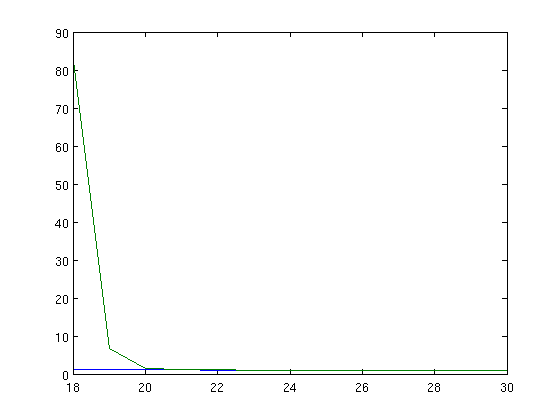
\includegraphics[scale=0.5]{images/2a.png}
\end{center}

\item $x \in [20,30]$ y N = 50


\begin{center}
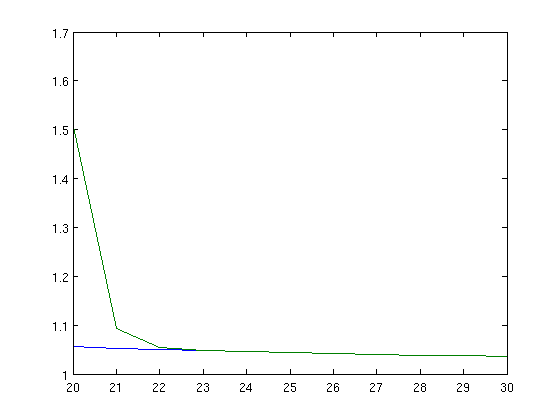
\includegraphics[scale=0.5]{images/2b.png}
\end{center}

\item $x \in [22,30]$ y N = 50


\begin{center}
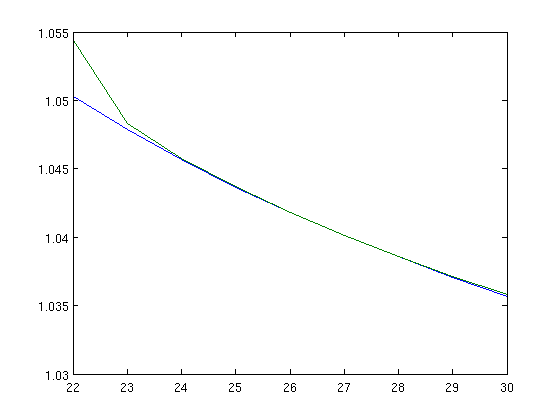
\includegraphics[scale=0.5]{images/2c.png}
\end{center}

\item $x \in [24,30]$ y N = 50

\begin{center}
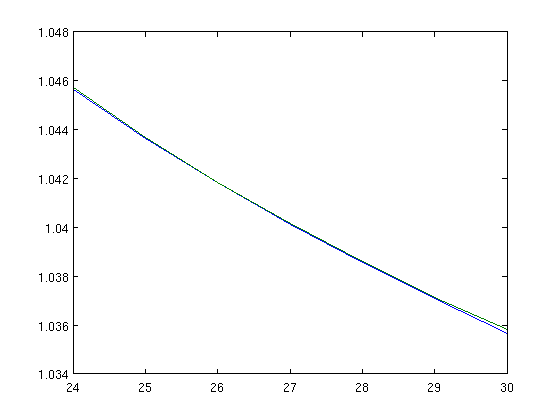
\includegraphics[scale=0.5]{images/2d.png}
\end{center}


Logrando finalmente darnos cuenta que para valores de x grandes:

$$
F(x) = x e^{-x} \sum_{n=1}^{\infty}\frac{x^n}{n(n!)} \thicksim 1 + \frac{1!}{x} + \frac{2!}{x^2} + \cdots
$$


\end{itemize}

La resolución más directa, consistiría en resolver la ecuación diferencial
ordinaria nombrada anteriormente computacionalmente. Esta solución es
fácilmente programable, y resolveria para pequeños y largos valores de $x$
limpiamente. La rutina automaticamente selecciona y ajusta la matriz en $x$
para proveer la presicion especificada y el detalle de la función. Lo único
que se debería analizar más a fondo sería los errores propagados e
inastibilidades de la ecuación diferencial en sí.

\newpage
\subsection{Integrales definidas}
En el presente trabajo, se toma como un nuevo ejemplo, una integral general definida de la forma:

\begin{eqnarray}
	I &=& \int_{a}^{b} f(t) dt
\end{eqnarray}

El enfoque estándar para realizar esta evaluación sería seleccionar primero una \emph{fórmula de cuadratura},
pero ¿Qué son las fórmulas de cuadraturas?.

Sea $f(x)$ una función continua definida en el intervalo $[a, b]$.
Nuestro objetivo será encontrar fórmulas aproximadas para calcular la integral $\int_{a}^{b}f(x) dx$.
En caso de conocer la primitiva $F(x)$ es evidente que podemos encontrar el valor exacto de la integral
utilizando el Teorema fundamental del cálculo integral: $\int_{a}^{b}f(x) dx = F(b) - F(a)$.
Sin embargo no siempre ésto es posible.

Por ejemplo, para la funcion $f(x) = e^{-x^{2}}$
no existe ninguna primitiva que podamos escribir utilizando funciones elementales.

Algunas fórmulas de cuadraturas son:
\begin{itemize}
	\item Fórmulas de los rectángulos.
	\item Fórmulas de  los trapecios.
	\item Método de Simpson.
	\item etc.
\end{itemize}

Volviendo a nuestro tema principal, el tipo de solución es normalmente realizado sobre la base de que conocemos
la primitiva, lo cual presenta una  facilidad de programación.
Entonces, se deben definir una malla adecuada de puntos para aplicar la fórmula de cuadratura.
El intervalo de malla seleccionado es casi siempre uniforme y acotado.

La principal dificultad asociada con este enfoque es, la determinación de un intervalo apropiado de integración.
Los límites de error habituales involucran las mayores derivadas de la función del integrando, $f(t)$.
Esta función suele ser tan complicada que un análisis de, por ejemplo, la quinta derivada es totalmente impracticable o,
por decir lo menos, poco economica.
Por la misma razón, es generalmente imposible especificar un intervalo variable de integración para aprovechar las
características variables de $f(t)$ sobre el intervalo de integración.

El método común para superar estas dificultades,
es llevar a cabo la integración dos veces con el doble del número de puntos en la segunda integración.
Luego, la precisión se puede afirmar, según el acuerdo de los dos resultados.
Una desventaja de este procedimiento es que un mínimo de tres veces más evaluaciones del integrando,
son necesarias como habría sido necesario un conocimiento a priori.
La necesidad práctica de utilizar una malla uniforme normalmente puede introducir un factor adicional de tres o cuatro.
Así que las evaluaciones más un orden de magnitud de la integral que se realizan son básicamente necesarias.
Este es un factor que no puede ser ignorado incluso en los computadores de hoy en día de alta velocidad.
Cabe señalar que en el caso de las integrales múltiples de orden N, esto se convierte en N órdenes de magnitud.

Un enfoque ``preferido'' es la de formar una ecuación diferencial mediante la definición de

\begin{eqnarray}
	I(x) = \int_{a}^{x} f(t) dt
\end{eqnarray}
y diferenciando
\begin{eqnarray}
	\frac{dI}{dx} = f(x),
\end{eqnarray}
con
\begin{eqnarray}
	I(a) = 0
\end{eqnarray}
entonces
\begin{eqnarray}
	I(b) = I
\end{eqnarray}

que sería igual que $(1)$, proporcionando el resultado deseado.
Debido a la naturaleza especial de la función derivada (sólo depende de x),
sólo una evaluación de la función es necesaria por paso, en lugar de dos para las derivadas de las funciones más general.
Una buena rutina de propósito general para las ecuaciones diferenciales contendrá los medios para tomar ventaja de este hecho.

Las ventajas de este enfoque es que la rutina de seguimiento continuo monitorea la presición de la integración y
aumenta el intervalo de integración, cuando sea posible.
Una malla variable apropiada es construida en línea con sólo una evaluación del integrando por cada paso,
mientras que la precisión adecuada se mantiene.
Un orden de magnitud en el tiempo de cálculo se obtiene de las integrales individuales;
dos órdenes de magnitud para las integrales dobles.

Este enfoque se pueden programar fácilmente y depurado.
Una vez más, una buena rutina de propósito general contiene los medios para asegurar que el punto final
(x = b) estará en la malla variable construida por la rutina.

\newpage
\subsection{Funciones especiales en el integrando}

Siguiendo la misma idea, podemos aprovechar ésta técnica para resolver
funciones especiales dentro de una integral. La idea es que sí estas funciones
especiales satisfacen una ecuación diferencial ordinaria, pueden ser
generadas por la solución de la ecuación diferencial definida.

Por ejemplo:

$$
	I	=	\int_0^\infty J_0 (t^2) e^{-t} dt
$$
\textit{(donde $J_0$ es la función regular cilindrica de Bessel de orden 0)}\\

Según lo visto al resolver integrales definidas, podemos hacer:
$$
	\frac{dI}{dx}	=	J_0 (x^2) e^{-x},
$$
con:
$$
	I(0) = 0
$$

Y el resultado deseado de $I(\infty) = I$.\\

Ahora normalmente uno podría proceder como ántes, y utilizar funciones de
Bessel\footnote{Son soluciones canonicas $y(x)$ de la ecuación diferencial de
Bessel: $x^2 \frac{d^2 y}{dx^2} + x \frac{dy}{dx} + (x^2 - \alpha^2)y = 0$}
 y subrutinas para la exponencial. Pero si suponemos por el momento que
no hay subrutinas para las funciones de Bessel en la biblioteca del programa,
podemos utilizar una alternativa a escribir la subrutina antes de resolver el
problema.

Ahora, está determinado (creánme) que $J_0(x^2)$ satisface la siguiente
ecuacion diferencial ordinaria de segundo orden:
$$
	\frac{d^2y}{dx^2} + (2 - \frac{1}{x}) \frac{dy}{dx} + 4x^2y = 0
$$
con 
$$
	y(0) = 1, \ \ \ \ \ \ \ \ \ \ \ \  y'(0) = 0
$$

Esta ecuación diferencial puede ser resuleta simultaneamente con el problema
anterior para evaluar la integral mientras generamos la función de Bessel
requerida. Específicamente, el problema completo es resuelto siguiendo el
siguiente sistema de ecuaciones de primer grado:

$$
	\frac{dI}{dx} = y_1 e^{-x}, \ \ \ \ \ \ \ \ \ \ \ \ \ \ \ I(0) = 0,
$$
$$
	\frac{dy_1}{dx} = y_2 ,\ \ \ \ \ \ \ \ \ \ \ \ \ \ \ \ \ \ y_1(0) = 1,
$$
$$
	\frac{dy_2}{dx} = \{^{-(2-\frac{1}{x})y_2-4x^2y_1 \ \ \ \ \ \ (x \neq
0)}_{0 \ \ \ \ \ \ \ \ \ \ \ \ \ \ \ \ \ \ \ \ \ \ (x = 0)}, \ \ \ y_2(0) = 0,
$$

Y se puede determinar facilmente un estimador del resto para proporcionar un
criterio para el término de la integración.

Esta última formulación del problema tiene varias ventajas:
\begin{enumerate}
	\item Evitamos la necesidad de escribri una subrutina especial para la
función de Bessel de esta aplicación en particular.
	\item La exactitud de los valores producidos por la función especial son
automáticamente monitoriades y son consistentes con la exactitud requerida
para la integral.
	\item Normalmente habrá menos tiempo de computación por cada evaluación de
la función en un factor de 4 o 5 más que la misma función evaluada por una
subrutina.
	\item Por último, habrá una ganacia en general por el acercamiento
realizado de un factor cerca de 25.
\end{enumerate}

Con la disponibilidad de una rutina de propósito general para la resolucion de
ecuaciones diferenciales ordinarias, la solución del sistema es fácilmente
programable y corregible.




\newpage
\subsection{Otras aplicaciones}

Las aplicaciones anteriores están destinadas a ser meramente ilustrativos, de poder resolver
el problema de una rutina de propósito general, para la solución de ecuaciones simultáneas
diferenciales ordinarias de primer orden. Ellos fueron seleccionados debido,
en parte, a que estaban entre los más evidentes de estas aplicaciones. Algunas
aplicaciones adicionales son las que nombraremos a continuación,
a modo de ejemplo, para indicar el mayor ámbito de aplicación de este enfoque general.
Existe cierta coincidencia en la lista, pero se cree mejor ser un poco
redundante a que, posiblemente, se le reste importancia a algunos temas.

\begin{enumerate}
	\item Múltiples integrales definidas\\
		Es evidente que los métodos de la sección 3 se puede generalizar para el
		tratamiento de las integrales múltiples. Las ventajas se multiplican en este caso,
		como se indica allí.

	\item Ecuaciones diferenciales derivadas en términos de un parámetro del
problema.\\
		En muchos casos, de decir, el rito esencial, es posible derivar una ecuación diferencial
		en función de un parámetro del problema y, posteriormente, resolver esta ecuación
		diferencial numéricamente (o, en casos excepcionales analíticamente!).
		Esto normalmente elimina toda una dimensión del problema.
		El ejemplo de la sección 2 es un ejemplo de esta técnica.		

	\item Ceros en funciones no-lineales (root-tracing) \\
		Una aplicación interesante de la técnica anterior se produce en la determinación de los loci
		de ceros de funciones no lineales.
		La información detallada en relación con este tema está disponible en $ [1] $.

	\item Equipotenciales, isotérmicos, campos lineales, etc.\\
		Las ecuaciones diferenciales de las curvas de los valores de la
		función constante pueden ser determinadas a través de la raíz de
		trazado de la técnica. Similares ecuaciones diferenciales
		para las trayectorias ortogonales también se obtiene fácilmente.

	\item  Derivadas dadas implícitamente en ecuaciones diferenciales
ordinarias.\\
		Las rutinas de propósito general están diseñados para resolver ecuaciones de la forma (1) con las
		expresiones derivadas dado de forma explícita. Si esto es imposible de alcanzar en una aplicación
		dada, por lo general hay alternativas. Las derivadas pueden ser la solución de un sistema lineal
		de ecuaciones algebraicas. En general, no se debe intentar producir las soluciones explícitas,
		sino más bien, el sistema lineal debe ser resuelto numéricamente en cada paso de integración.
		Si el derivado se da implícitamente en forma no lineal $G(x,y,y') = 0$, la técnica de trazado
		de la raíz puede ser utilizado para producir una solución en línea de la ecuación no lineal.

	\item Integrales oscilatorios.\\
		Graves dificultades de computación se producen cuando el integrando de una integral es muy oscilante.
		En algunos casos, es imposible obtener resultados significativos en todos los de una integración directa.
		Una técnica eficaz para el alivio de esta dificultad es deformar el camino de la integración en el plano
		complejo. Lo que se desea es el camino de integración de arte que a lo largo de la fase de la función
		integrando es constante. La raíz de la técnica de rastreo permite la determinación simultánea de la ruta
		adecuada de la integración, junto con la integración en sí, ver $[2]$.

	\item Problemas del valor de dos puntos de la frontera.\\
		Dos problemas de límite de valor de punto se suelen resolverse a través de la solución iterativa de
		problemas de valor inicial. Algunas técnicas que giran alrededor de la solución simultánea de las ecuaciones
		diferenciales relacionadas con acelerar el proceso de convergencia, véase $[3]$. Más significativamente,
		a veces es posible reducir el problema a un problema de valor inicial en un parámetro del problema, ver $[4]$.

	\item Ecuaciones diferenciales parciales parabólicas y hiperbólicas.\\
		En la ``marcha de tipo'' problemas de ecuaciones diferenciales parciales a menudo es conveniente para
		discretizar una o más (por lo general el espacio), pero las variables de mecanización de la marcha variable
		(normalmente el tiempo) a través de una rutina de propósito general para la solución de ecuaciones diferenciales
		ordinarias simultáneas. Se obtiene un número de sistemas de ecuaciones diferenciales ordinarias igual al número
		de puntos de malla en las variables de espacio.

	\item Ecuaciones Integrales.\\
		Muchos de los problemas expresados en términos de las ecuaciones integrales tienen representaciones equivalentes
		en términos de ecuaciones diferenciales. Esta última forma es a menudo superior desde un punto de vista de la
		informática.

\end{enumerate}

\newpage

\section{Conclusiones}
Se ha hecho aquí un intento, para crear un caso para resolver el gran problema de alimentación
de la rutina para la solución de sistemas de ecuaciones diferenciales ordinarias simultáneas.
 Esta tesis que hemos estudiado, tiene una sólida base en la experiencia
operativa del Grupo de Matemática Aplicada en los Laboratorios RCA en Princeton, Nueva Jersey.
Las rutinas que estudiamos, contienen múltiples ventajas del control
automática de errores y modificación del intervalo, y se considera
que incluso superan a las ventajas aparentes de la cuadratura de Gauss.
 Esto en sí mismo era suficiente para el procesamiento de una gran clase de
problemas.

Los ejemplos anteriores demuestran que muchos problemas pueden ser expresados en términos de la solución
de sistemas de ecuaciones diferenciales ordinarias simultáneas. Una buena rutina de propósito general
para la solución de estos sistemas proporciona una poderosa herramienta para el procesamiento de estos
problemas. Esto es cierto desde el punto de vista de la facilidad de la programación, la facilidad de
depuración y reducción al mínimo de tiempo de computadora.

\newpage

\section{Glosario}
\begin{description}
	\item[Función de Bessel]
	Son soluciones canonicas $y(x)$ de la ecuación diferencial de
Bessel:
$$
x^2 \frac{d^2 y}{dx^2} + x \frac{dy}{dx} + (x^2 - \alpha^2)y = 0
$$
	\item[$J_0$]
	Función de Bessel de primera especie y orden 0. Para las soluciones de orden entero es
posible definir la función $J_0(x)$ por su expansión en serie de Taylor en
torno a $x = 0$:
$$
J_0(x)= 1-\frac{x^2}{2^2}+\frac{x^4}{2^2 4^2}-\frac{x^6}{2^2 4^2 6^2}\ldots
$$
$$
J'_0(x)= \frac{dJ_0(x)}{dx} = -J_1(x)
$$

	\item[Función continua]
	Una función $f$ es continua en el punto $a$, si $f$ está definida en algún intervalo abierto que contenga
	a $a$ y si para cualquier $\epsilon > 0$ existe un $\delta > 0$ tal que:
	$$si\ |x-a| > \delta\ entonces\ |f(x)-f(a)|< \epsilon$$
	
	\item [Malla]
	La malla de la partición:
	$$x_0 < x_1 < x_2 < \ldots < x_n$$
	es el largo del subintervalo mas largo:
	$$max|x_i - x_{i-1}|: i=1\ldots n$$
	Si la malla tiende a cero, podemos tener una suma de Riemann, lo que conlleva a una integral de Riemann.

\end{description}

\newpage

%\section{Anexos}
%\input{src/8-anexos}
%\newpage

\bibliography{informe}

\end{document}
